\documentclass[]{article}
\usepackage{lmodern}
\usepackage{amssymb,amsmath}
\usepackage{ifxetex,ifluatex}
\usepackage{fixltx2e} % provides \textsubscript
\ifnum 0\ifxetex 1\fi\ifluatex 1\fi=0 % if pdftex
  \usepackage[T1]{fontenc}
  \usepackage[utf8]{inputenc}
\else % if luatex or xelatex
  \ifxetex
    \usepackage{mathspec}
  \else
    \usepackage{fontspec}
  \fi
  \defaultfontfeatures{Ligatures=TeX,Scale=MatchLowercase}
\fi
% use upquote if available, for straight quotes in verbatim environments
\IfFileExists{upquote.sty}{\usepackage{upquote}}{}
% use microtype if available
\IfFileExists{microtype.sty}{%
\usepackage{microtype}
\UseMicrotypeSet[protrusion]{basicmath} % disable protrusion for tt fonts
}{}
\usepackage[margin=1in]{geometry}
\usepackage{hyperref}
\hypersetup{unicode=true,
            pdftitle={NZ GREEN Grid Household Power Demand Profiles: Heat Pump},
            pdfauthor={Ben Anderson (b.anderson@soton.ac.uk, @dataknut)},
            pdfborder={0 0 0},
            breaklinks=true}
\urlstyle{same}  % don't use monospace font for urls
\usepackage{color}
\usepackage{fancyvrb}
\newcommand{\VerbBar}{|}
\newcommand{\VERB}{\Verb[commandchars=\\\{\}]}
\DefineVerbatimEnvironment{Highlighting}{Verbatim}{commandchars=\\\{\}}
% Add ',fontsize=\small' for more characters per line
\usepackage{framed}
\definecolor{shadecolor}{RGB}{248,248,248}
\newenvironment{Shaded}{\begin{snugshade}}{\end{snugshade}}
\newcommand{\KeywordTok}[1]{\textcolor[rgb]{0.13,0.29,0.53}{\textbf{#1}}}
\newcommand{\DataTypeTok}[1]{\textcolor[rgb]{0.13,0.29,0.53}{#1}}
\newcommand{\DecValTok}[1]{\textcolor[rgb]{0.00,0.00,0.81}{#1}}
\newcommand{\BaseNTok}[1]{\textcolor[rgb]{0.00,0.00,0.81}{#1}}
\newcommand{\FloatTok}[1]{\textcolor[rgb]{0.00,0.00,0.81}{#1}}
\newcommand{\ConstantTok}[1]{\textcolor[rgb]{0.00,0.00,0.00}{#1}}
\newcommand{\CharTok}[1]{\textcolor[rgb]{0.31,0.60,0.02}{#1}}
\newcommand{\SpecialCharTok}[1]{\textcolor[rgb]{0.00,0.00,0.00}{#1}}
\newcommand{\StringTok}[1]{\textcolor[rgb]{0.31,0.60,0.02}{#1}}
\newcommand{\VerbatimStringTok}[1]{\textcolor[rgb]{0.31,0.60,0.02}{#1}}
\newcommand{\SpecialStringTok}[1]{\textcolor[rgb]{0.31,0.60,0.02}{#1}}
\newcommand{\ImportTok}[1]{#1}
\newcommand{\CommentTok}[1]{\textcolor[rgb]{0.56,0.35,0.01}{\textit{#1}}}
\newcommand{\DocumentationTok}[1]{\textcolor[rgb]{0.56,0.35,0.01}{\textbf{\textit{#1}}}}
\newcommand{\AnnotationTok}[1]{\textcolor[rgb]{0.56,0.35,0.01}{\textbf{\textit{#1}}}}
\newcommand{\CommentVarTok}[1]{\textcolor[rgb]{0.56,0.35,0.01}{\textbf{\textit{#1}}}}
\newcommand{\OtherTok}[1]{\textcolor[rgb]{0.56,0.35,0.01}{#1}}
\newcommand{\FunctionTok}[1]{\textcolor[rgb]{0.00,0.00,0.00}{#1}}
\newcommand{\VariableTok}[1]{\textcolor[rgb]{0.00,0.00,0.00}{#1}}
\newcommand{\ControlFlowTok}[1]{\textcolor[rgb]{0.13,0.29,0.53}{\textbf{#1}}}
\newcommand{\OperatorTok}[1]{\textcolor[rgb]{0.81,0.36,0.00}{\textbf{#1}}}
\newcommand{\BuiltInTok}[1]{#1}
\newcommand{\ExtensionTok}[1]{#1}
\newcommand{\PreprocessorTok}[1]{\textcolor[rgb]{0.56,0.35,0.01}{\textit{#1}}}
\newcommand{\AttributeTok}[1]{\textcolor[rgb]{0.77,0.63,0.00}{#1}}
\newcommand{\RegionMarkerTok}[1]{#1}
\newcommand{\InformationTok}[1]{\textcolor[rgb]{0.56,0.35,0.01}{\textbf{\textit{#1}}}}
\newcommand{\WarningTok}[1]{\textcolor[rgb]{0.56,0.35,0.01}{\textbf{\textit{#1}}}}
\newcommand{\AlertTok}[1]{\textcolor[rgb]{0.94,0.16,0.16}{#1}}
\newcommand{\ErrorTok}[1]{\textcolor[rgb]{0.64,0.00,0.00}{\textbf{#1}}}
\newcommand{\NormalTok}[1]{#1}
\usepackage{graphicx,grffile}
\makeatletter
\def\maxwidth{\ifdim\Gin@nat@width>\linewidth\linewidth\else\Gin@nat@width\fi}
\def\maxheight{\ifdim\Gin@nat@height>\textheight\textheight\else\Gin@nat@height\fi}
\makeatother
% Scale images if necessary, so that they will not overflow the page
% margins by default, and it is still possible to overwrite the defaults
% using explicit options in \includegraphics[width, height, ...]{}
\setkeys{Gin}{width=\maxwidth,height=\maxheight,keepaspectratio}
\IfFileExists{parskip.sty}{%
\usepackage{parskip}
}{% else
\setlength{\parindent}{0pt}
\setlength{\parskip}{6pt plus 2pt minus 1pt}
}
\setlength{\emergencystretch}{3em}  % prevent overfull lines
\providecommand{\tightlist}{%
  \setlength{\itemsep}{0pt}\setlength{\parskip}{0pt}}
\setcounter{secnumdepth}{5}
% Redefines (sub)paragraphs to behave more like sections
\ifx\paragraph\undefined\else
\let\oldparagraph\paragraph
\renewcommand{\paragraph}[1]{\oldparagraph{#1}\mbox{}}
\fi
\ifx\subparagraph\undefined\else
\let\oldsubparagraph\subparagraph
\renewcommand{\subparagraph}[1]{\oldsubparagraph{#1}\mbox{}}
\fi

%%% Use protect on footnotes to avoid problems with footnotes in titles
\let\rmarkdownfootnote\footnote%
\def\footnote{\protect\rmarkdownfootnote}

%%% Change title format to be more compact
\usepackage{titling}

% Create subtitle command for use in maketitle
\newcommand{\subtitle}[1]{
  \posttitle{
    \begin{center}\large#1\end{center}
    }
}

\setlength{\droptitle}{-2em}
  \title{NZ GREEN Grid Household Power Demand Profiles: Heat Pump}
  \pretitle{\vspace{\droptitle}\centering\huge}
  \posttitle{\par}
\subtitle{Data extraction and preliminary plots}
  \author{Ben Anderson
(\href{mailto:b.anderson@soton.ac.uk}{\nolinkurl{b.anderson@soton.ac.uk}},
\texttt{@dataknut})}
  \preauthor{\centering\large\emph}
  \postauthor{\par}
  \predate{\centering\large\emph}
  \postdate{\par}
  \date{Last run at: 2018-06-08 11:39:08}


\begin{document}
\maketitle

{
\setcounter{tocdepth}{2}
\tableofcontents
}
\newpage

\section{Status}\label{status}

Full run using all data from /Volumes/hum-csafe/Research Projects/GREEN
Grid/\_RAW DATA/GridSpyData/

\section{Citation}\label{citation}

If you wish to use any of the material from this report please cite as:

\begin{itemize}
\tightlist
\item
  Anderson, B. (2018) GREEN Grid Heat Pump Profiles, University of
  Otago: Dunedin, NZ.
\end{itemize}

\newpage

\section{Introduction}\label{introduction}

Report circulation:

\begin{itemize}
\tightlist
\item
  Restricted to:
  \href{https://www.otago.ac.nz/centre-sustainability/research/energy/otago050285.html}{NZ
  GREEN Grid} project partners and contractors.
\end{itemize}

\subsection{Purpose}\label{purpose}

This report is intended to:

\begin{itemize}
\tightlist
\item
  load and clean the project electricity power data (Grid Spy)
\item
  select the Heat Pump circuits (via their labels)
\item
  build exploratory demand profiles
\end{itemize}

\subsection{Requirements:}\label{requirements}

\begin{itemize}
\tightlist
\item
  cleaned and safe grid spy 1 minute data processed via
  \url{https://git.soton.ac.uk/ba1e12/nzGREENGrid/blob/master/dataProcessing/processNZGGElecCons1minData.Rmd}
\end{itemize}

\subsection{History}\label{history}

Generally tracked via our git.soton
\href{https://git.soton.ac.uk/ba1e12/nzGREENGrid}{repo}:

\begin{itemize}
\tightlist
\item
  \href{https://git.soton.ac.uk/ba1e12/nzGREENGrid/commits/master}{history}
\item
  \href{https://git.soton.ac.uk/ba1e12/nzGREENGrid/issues}{issues}
\end{itemize}

\subsection{Support}\label{support}

This work was supported by:

\begin{itemize}
\tightlist
\item
  The \href{https://www.otago.ac.nz/}{University of Otago}
\item
  The New Zealand \href{http://www.mbie.govt.nz/}{Ministry of Business,
  Innovation and Employment (MBIE)}
\item
  \href{http://www.energy.soton.ac.uk/tag/spatialec/}{SPATIALEC} - a
  \href{http://ec.europa.eu/research/mariecurieactions/about-msca/actions/if/index_en.htm}{Marie
  Skłodowska-Curie Global Fellowship} based at the University of Otago's
  \href{http://www.otago.ac.nz/centre-sustainability/staff/otago673896.html}{Centre
  for Sustainability} (2017-2019) \& the University of Southampton's
  Sustainable Energy Research Group (2019-202).
\end{itemize}

This work is (c) 2018 the University of Southampton.

We do not `support' the code but if you have a problem check the
\href{https://git.soton.ac.uk/ba1e12/nzGREENGrid/issues}{issues} on our
\href{https://git.soton.ac.uk/ba1e12/nzGREENGrid}{repo} and if it
doesn't already exist, open one. We might be able to fix it :-)

\section{Load data files}\label{load-data-files}

\subsection{Grid Spy metadata}\label{grid-spy-metadata}

In this section we load metadata from /Users/ben/Syncplicity
Folders/Green Grid Project Management Folder/Gridspy/Master list of
Gridspy units.xlsx to link to the power data.

\begin{verbatim}
##    sample  hhID          Adults Teenagers             Children removed
## 1: Unison rf_28               2      <NA>            3(12,8,4)    <NA>
## 2: Unison rf_29               2      <NA>     1 (7 months old)    live
## 3: Unison rf_30               2         0                    0    <NA>
## 4: Unison rf_31 2 (Plus cousin)      <NA>                 <NA>    live
## 5: Unison rf_32               2      <NA> 2 (7 and 4years old)    <NA>
## 6: Unison rf_33               2 1(14yold)            1 (6yold)    live
\end{verbatim}

\begin{verbatim}
##     sample  hhID Adults Teenagers Children  removed
## 1: Powerco rf_12      1      <NA>     <NA> 3/6/1015
## 2: Powerco  <NA>      1      <NA>     <NA>     <NA>
## 3: Powerco rf_25      1      <NA>     <NA>     <NA>
## 4: Powerco  <NA>     NA      <NA>     <NA>     <NA>
## 5: Powerco  <NA>      1      <NA>   1(5mo)     <NA>
## 6: Powerco  <NA>     NA      <NA>     <NA>     <NA>
\end{verbatim}

Meta data for sample

sample

hhID

Adults

Teenagers

Children

removed

nAdults

Powerco

rf\_06

2

NA

NA

NA

2

Powerco

rf\_07

2

NA

2

NA

2

Powerco

rf\_08

2

NA

NA

NA

2

Powerco

rf\_09

2

NA

1

42171

2

Powerco

rf\_10

2

NA

1(3yo)

NA

3

Powerco

rf\_11

NA

NA

NA

NA

1

Powerco

rf\_12

1

NA

NA

3/6/1015

1

Powerco

rf\_13

2

1(16yo)

1(11)

NA

2

Powerco

rf\_14

1

NA

1 (11 yo)

NA

1

Powerco

rf\_15

NA

NA

NA

42462

1

Powerco

rf\_15\_old

1

NA

NA

42019

1

Powerco

rf\_16

2

NA

NA

42089

2

Powerco

rf\_17 sn\_662

NA

NA

NA

NA

1

Powerco

rf\_17\_oldNo reused

2

1(13yo)

1(11yo)

42457

2

Powerco

rf\_18

2

NA

1(1yo)

42532

2

Powerco

rf\_19

1

NA

NA

NA

1

Powerco

rf\_20

2

NA

2

42166

2

Powerco

rf\_21

2

NA

NA

42821

2

Powerco

rf\_22

2

NA

NA

NA

2

Powerco

rf\_23

1

NA

NA

NA

1

Powerco

rf\_24

2

NA

2

NA

2

Powerco

rf\_25

1

NA

NA

NA

1

Powerco

rf\_26

2

NA

NA

NA

2

Powerco

rf\_27

2

1

1

NA

2

Unison

rf\_28

2

NA

3(12,8,4)

NA

3

Unison

rf\_29

2

NA

1 (7 months old)

live

2

Unison

rf\_30

2

0

0

NA

2

Unison

rf\_31

2 (Plus cousin)

NA

NA

live

2

Unison

rf\_32

2

NA

2 (7 and 4years old)

NA

2

Unison

rf\_33

2

1(14yold)

1 (6yold)

live

2

Unison

rf\_34

3

NA

NA

NA

1

Unison

rf\_35

2

NA

NA

42322

2

Unison

rf\_36

1

2 (14 and 12)

NA

live

1

Unison

rf\_37

2

NA

NA

live

2

Unison

rf\_38

NA

NA

NA

NA

1

Unison

rf\_38

2

NA

2 (\textless{}12)

NA

2

Unison

rf\_39

2

1 (16 YO)

NA

live

2

Unison

rf\_40

2

NA

NA

42330

2

Unison

rf\_41

2

NA

2 (11 and 8)

live

2

Unison

rf\_42

2

NA

3 (\textless{}12 yold, 1 10 YO)

NA

3

Unison

rf\_43

2

NA

NA

42296

2

Unison

rf\_44

2

NA

2 (10 and 7)

NA

2

Unison

rf\_45

2

NA

3 (\textless{}12 years old)

NA

3

Unison

rf\_46

2

NA

1 (4yold-50\%)

live

2

Unison

rf\_47

3

2

NA

NA

1

\subsection{Grid Spy data}\label{grid-spy-data}

In this section we load the cleaned data files from
/Volumes/hum-csafe/Research Projects/GREEN
Grid/Clean\_data/safe/gridSpy/1min/data/. If we loaded all the data at
once and then filtered out what we want we might run out of memory so we
filter as we load. Set the filters here:

\begin{Shaded}
\begin{Highlighting}[]
\NormalTok{circuitPattern <-}\StringTok{ }\NormalTok{params}\OperatorTok{$}\NormalTok{circuitPattern}
\NormalTok{dateFrom <-}\StringTok{ }\NormalTok{params}\OperatorTok{$}\NormalTok{dateFrom}
\NormalTok{dateTo <-}\StringTok{ }\NormalTok{params}\OperatorTok{$}\NormalTok{dateTo}

\NormalTok{plotCaption <-}\StringTok{ }\KeywordTok{paste0}\NormalTok{(}\StringTok{"Source: "}\NormalTok{, fpath,}
                      \StringTok{"}\CharTok{\textbackslash{}n}\StringTok{Circuits: "}\NormalTok{, circuitPattern, }\StringTok{" from "}\NormalTok{, dateFrom, }\StringTok{" to "}\NormalTok{, dateTo)}
\end{Highlighting}
\end{Shaded}

So we are looking for Heat Pump circuits between 2015-04-01 and
2016-03-31. We do this by checking to see if the extract file has
already been created. If so we load it. If not, we create it.

The file we are looking for is: Heat
Pump\_2015-04-01\_2016-03-31\_observations.csv

\begin{verbatim}
## [1] "/Volumes/hum-csafe/Research Projects/GREEN Grid/Clean_data/safe/gridSpy/1min/dataExtracts/Heat Pump_2015-04-01_2016-03-31_observations.csv exists so re-loading..."
## [1] "# Loaded 14,252,439 rows of data"
\end{verbatim}

The following table summarises the Heat Pump data we have found.

Summary of household grid spy data for: Heat Pump

hhID

nObs

nHouseholds

nCircuits

meanPower

minDate

maxDate

rf\_08

521843

1

1

65.92309

2015-04-01

2016-03-31

rf\_09

152669

1

1

266.37950

2015-04-01

2015-07-16

rf\_10

526797

1

1

52.40885

2015-04-01

2016-03-31

rf\_11

519185

1

1

236.23474

2015-04-01

2016-03-31

rf\_13

1053858

1

2

227.22865

2015-04-01

2016-03-31

rf\_17

520028

1

1

31.15216

2015-04-01

2016-03-28

rf\_19

1053136

1

2

39.53314

2015-04-01

2016-03-31

rf\_20

102188

1

1

140.09662

2015-04-01

2015-06-11

rf\_21

505042

1

1

118.65538

2015-04-01

2016-03-31

rf\_25

443936

1

1

67.43931

2015-05-24

2016-03-31

rf\_27

497806

1

1

168.10637

2015-04-01

2016-03-31

rf\_28

79085

1

1

56.43806

2015-04-01

2015-05-26

rf\_29

526780

1

1

646.73224

2015-04-01

2016-03-31

rf\_31

526878

1

1

95.06807

2015-04-01

2016-03-31

rf\_32

526785

1

1

69.66461

2015-04-01

2016-03-31

rf\_33

526863

1

1

359.19048

2015-04-01

2016-03-31

rf\_34

526677

1

1

174.28675

2015-04-01

2016-03-31

rf\_35

327974

1

1

79.08711

2015-04-01

2015-11-14

rf\_36

516242

1

1

76.00384

2015-04-01

2016-03-31

rf\_37

526771

1

1

75.30394

2015-04-01

2016-03-31

rf\_38

373722

1

1

282.16696

2015-04-01

2015-12-26

rf\_40

338289

1

1

336.91930

2015-04-01

2015-11-22

rf\_41

223824

1

1

82.65447

2015-04-01

2015-11-12

rf\_42

518179

1

1

48.25356

2015-04-01

2016-03-31

rf\_43

288838

1

1

200.56165

2015-04-01

2015-10-18

rf\_44

526850

1

1

109.39986

2015-04-01

2016-03-31

rf\_45

526110

1

1

85.44295

2015-04-01

2016-03-31

rf\_46

950976

1

2

90.78617

2015-04-01

2016-03-31

rf\_47

525108

1

1

132.97838

2015-04-01

2016-03-31

This table will have a large number (14,252,439) of obserations caused
by the number of different circuit labels as shown by the following
table.

Counts of Heat Pump observations by label and household

rf\_08

rf\_09

rf\_10

rf\_11

rf\_13

rf\_17

rf\_19

rf\_20

rf\_21

rf\_25

rf\_27

rf\_28

rf\_29

rf\_31

rf\_32

rf\_33

rf\_34

rf\_35

rf\_36

rf\_37

rf\_38

rf\_40

rf\_41

rf\_42

rf\_43

rf\_44

rf\_45

rf\_46

rf\_47

Bedroom \& Lounge Heat Pumps\$2741

0

0

0

0

0

0

526568

0

0

0

0

0

0

0

0

0

0

0

0

0

0

0

0

0

0

0

0

0

0

Downstairs (inc 1 Heat Pump)\$2212

0

0

0

0

526929

0

0

0

0

0

0

0

0

0

0

0

0

0

0

0

0

0

0

0

0

0

0

0

0

Heat Pump (x2) \& Lounge Power\$4166

0

0

0

0

0

0

0

0

0

0

0

0

0

0

0

0

0

0

0

0

0

338289

0

0

0

0

0

0

0

Heat Pump \& 2 x Bathroom Heat\$4171

0

0

0

0

0

0

0

0

0

0

0

0

0

0

0

0

0

0

0

0

0

0

0

0

0

0

0

0

525108

Heat Pump \& Bedroom 2\$2731

0

152669

0

0

0

0

0

0

0

0

0

0

0

0

0

0

0

0

0

0

0

0

0

0

0

0

0

0

0

Heat Pump \& Kitchen Appliances\$4186

0

0

0

0

0

0

0

0

0

0

0

0

526780

0

0

0

0

0

0

0

0

0

0

0

0

0

0

0

0

Heat Pump \& Lounge\$2590

0

0

0

519185

0

0

0

0

0

0

0

0

0

0

0

0

0

0

0

0

0

0

0

0

0

0

0

0

0

Heat Pump \& Misc\$2107

0

0

0

0

0

0

0

102188

0

0

0

0

0

0

0

0

0

0

0

0

0

0

0

0

0

0

0

0

0

Heat Pump \& Washing Machine\$2750

0

0

0

0

0

0

0

0

505042

0

0

0

0

0

0

0

0

0

0

0

0

0

0

0

0

0

0

0

0

Heat Pump\$2092

521843

0

0

0

0

0

0

0

0

0

0

0

0

0

0

0

0

0

0

0

0

0

0

0

0

0

0

0

0

Heat Pump\$2148

0

0

0

0

0

520028

0

0

0

0

0

0

0

0

0

0

0

0

0

0

0

0

0

0

0

0

0

0

0

Heat Pump\$2598

0

0

526797

0

0

0

0

0

0

0

0

0

0

0

0

0

0

0

0

0

0

0

0

0

0

0

0

0

0

Heat Pump\$2758

0

0

0

0

0

0

0

0

0

443936

0

0

0

0

0

0

0

0

0

0

0

0

0

0

0

0

0

0

0

Heat Pump\$2826

0

0

0

0

0

0

0

0

0

0

497806

0

0

0

0

0

0

0

0

0

0

0

0

0

0

0

0

0

0

Heat Pump\$4124

0

0

0

0

0

0

0

0

0

0

0

0

0

0

0

0

0

327974

0

0

0

0

0

0

0

0

0

0

0

Heat Pump\$4130

0

0

0

0

0

0

0

0

0

0

0

0

0

0

0

0

0

0

0

0

0

0

0

518179

0

0

0

0

0

Heat Pump\$4134

0

0

0

0

0

0

0

0

0

0

0

0

0

0

0

0

0

0

0

526771

0

0

0

0

0

0

0

0

0

Heat Pump\$4150

0

0

0

0

0

0

0

0

0

0

0

0

0

0

0

0

0

0

516242

0

0

0

0

0

0

0

0

0

0

Heat Pump\$4154

0

0

0

0

0

0

0

0

0

0

0

0

0

0

0

0

0

0

0

0

0

0

0

0

0

526850

0

0

0

Heat Pump\$4160

0

0

0

0

0

0

0

0

0

0

0

0

0

0

0

0

0

0

0

0

0

0

0

0

0

0

526110

0

0

Heat Pump\$4175

0

0

0

0

0

0

0

0

0

0

0

0

0

0

0

0

0

0

0

0

373722

0

0

0

0

0

0

0

0

Heat Pump\$4190

0

0

0

0

0

0

0

0

0

0

0

0

0

0

0

0

0

0

0

0

0

0

223824

0

0

0

0

0

0

Heat Pump\$4196

0

0

0

0

0

0

0

0

0

0

0

0

0

0

526785

0

0

0

0

0

0

0

0

0

0

0

0

0

0

Heat Pump\$4204

0

0

0

0

0

0

0

0

0

0

0

0

0

526878

0

0

0

0

0

0

0

0

0

0

0

0

0

0

0

Heat Pump\$4211

0

0

0

0

0

0

0

0

0

0

0

0

0

0

0

0

0

0

0

0

0

0

0

0

288838

0

0

0

0

Heat Pump\$4219

0

0

0

0

0

0

0

0

0

0

0

79085

0

0

0

0

0

0

0

0

0

0

0

0

0

0

0

0

0

Heat Pump\$4223

0

0

0

0

0

0

0

0

0

0

0

0

0

0

0

0

526677

0

0

0

0

0

0

0

0

0

0

0

0

Heat Pumps (2x) \& Power\$4232

0

0

0

0

0

0

0

0

0

0

0

0

0

0

0

0

0

0

0

0

0

0

0

0

0

0

0

486982

0

Heat Pumps (2x) \& Power\$4399

0

0

0

0

0

0

0

0

0

0

0

0

0

0

0

0

0

0

0

0

0

0

0

0

0

0

0

463994

0

Kitchen Appliances \& Heat Pump\$4140

0

0

0

0

0

0

0

0

0

0

0

0

0

0

0

526863

0

0

0

0

0

0

0

0

0

0

0

0

0

Theatre Heat Pump\$2740

0

0

0

0

0

0

526568

0

0

0

0

0

0

0

0

0

0

0

0

0

0

0

0

0

0

0

0

0

0

Upstairs Heat Pumps\$2211

0

0

0

0

526929

0

0

0

0

0

0

0

0

0

0

0

0

0

0

0

0

0

0

0

0

0

0

0

0

Note that some households may have more than one Heat Pump circuit.

\subsection{Test Heat Pump data}\label{test-heat-pump-data}

This section tests the availability of Heat Pump data by replicating the
standard data quality checks used for the whole
\href{https://git.soton.ac.uk/ba1e12/nzGREENGrid/tree/master/dataProcessing/gridSpy}{gridSpy
dataset}.

The following plot shows loaded data observation plots - just to confirm
what Heat Pump data we have.

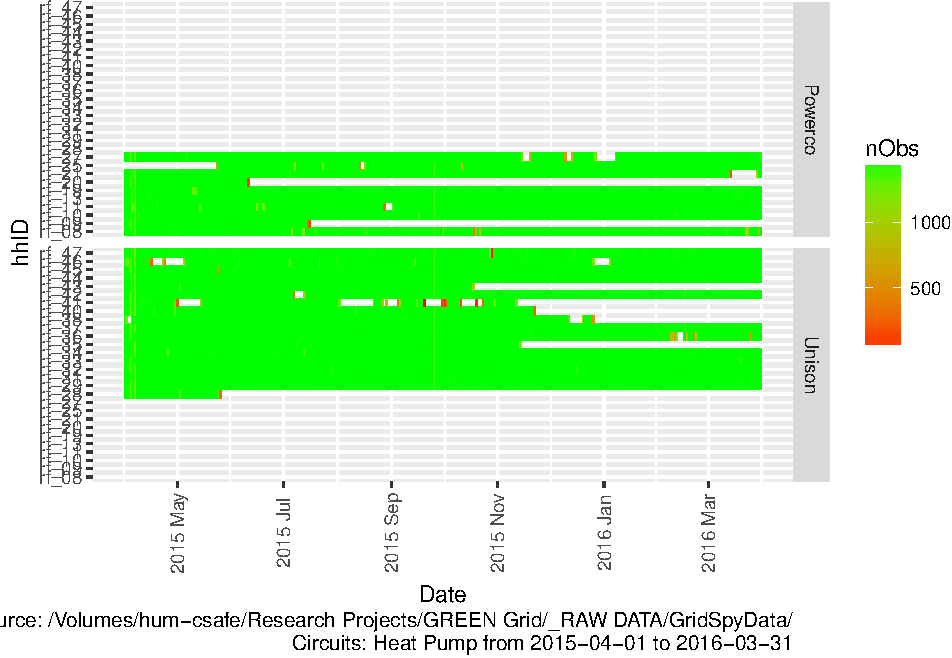
\includegraphics{ggProfile_Heat Pump_2015-04-01_2016-03-31_files/figure-latex/loadedFilesObs Tile Plot-1.pdf}

The next plot shows the same data but as a dot plot to highlight those
households and dates where we did not receive 60 * 24 = 1440
observations per day.

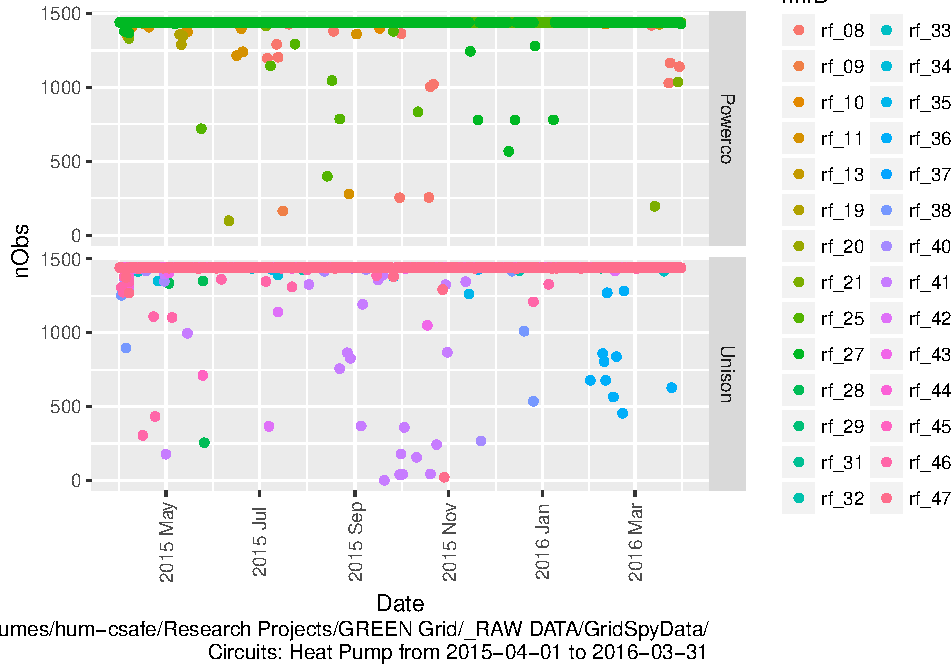
\includegraphics{ggProfile_Heat Pump_2015-04-01_2016-03-31_files/figure-latex/loadedFilesObs point plot-1.pdf}

The following table shows the min/max observations per day and min/max
dates for each household. As above, we should not see:

\begin{itemize}
\tightlist
\item
  dates before 2014 or in to the future (indicates date conversion
  errors)
\item
  more than 1440 observations per day (indicates potentially duplicate
  observations)
\item
  non-integer counts of circuits as it suggests some column errors
\end{itemize}

We should also not see NA in any row (indicates date conversion errors).

If we do see any of these then we still have data cleaning work to do!

Summary observation stats by hhID (sorted by date last heard from) for:
Heat Pump

hhID

sample

nObs

minDate

maxDate

rf\_28

Unison

79085

2015-04-01T00:00:00Z

2015-05-26T04:56:00Z

rf\_20

Powerco

102188

2015-04-01T00:00:00Z

2015-06-11T01:37:00Z

rf\_09

Powerco

152669

2015-04-01T00:00:00Z

2015-07-16T02:42:00Z

rf\_43

Unison

288838

2015-04-01T00:00:00Z

2015-10-18T17:29:00Z

rf\_41

Unison

223824

2015-04-01T00:00:00Z

2015-11-12T22:24:00Z

rf\_35

Unison

327974

2015-04-01T00:00:00Z

2015-11-14T21:00:00Z

rf\_40

Unison

338289

2015-04-01T00:00:00Z

2015-11-22T04:27:00Z

rf\_38

Unison

747444

2015-04-01T00:00:00Z

2015-12-26T08:55:00Z

rf\_08

Powerco

521843

2015-04-01T00:00:00Z

2016-03-31T23:59:00Z

rf\_10

Powerco

526797

2015-04-01T00:00:00Z

2016-03-31T23:59:00Z

rf\_11

Powerco

519185

2015-04-01T00:00:00Z

2016-03-31T23:59:00Z

rf\_13

Powerco

1053858

2015-04-01T00:00:00Z

2016-03-31T23:59:00Z

rf\_19

Powerco

1053136

2015-04-01T00:00:00Z

2016-03-31T23:59:00Z

rf\_21

Powerco

505042

2015-04-01T00:00:00Z

2016-03-31T23:59:00Z

rf\_25

Powerco

443936

2015-05-24T12:00:00Z

2016-03-31T23:59:00Z

rf\_27

Powerco

497806

2015-04-01T00:00:00Z

2016-03-31T23:59:00Z

rf\_29

Unison

526780

2015-04-01T00:00:00Z

2016-03-31T23:59:00Z

rf\_31

Unison

526878

2015-04-01T00:00:00Z

2016-03-31T23:59:00Z

rf\_32

Unison

526785

2015-04-01T00:00:00Z

2016-03-31T23:59:00Z

rf\_33

Unison

526863

2015-04-01T00:00:00Z

2016-03-31T23:59:00Z

rf\_34

Unison

526677

2015-04-01T00:00:00Z

2016-03-31T23:59:00Z

rf\_36

Unison

516242

2015-04-01T00:00:00Z

2016-03-31T23:59:00Z

rf\_37

Unison

526771

2015-04-01T00:00:00Z

2016-03-31T23:59:00Z

rf\_42

Unison

518179

2015-04-01T00:00:00Z

2016-03-31T23:59:00Z

rf\_44

Unison

526850

2015-04-01T00:00:00Z

2016-03-31T23:59:00Z

rf\_45

Unison

526110

2015-04-01T00:00:00Z

2016-03-31T23:59:00Z

rf\_46

Unison

950976

2015-04-01T00:00:00Z

2016-03-31T23:59:00Z

rf\_47

Unison

525108

2015-04-01T00:00:00Z

2016-03-31T23:59:00Z

Finally we show the total number of households which we think we have
Heat Pump data for.

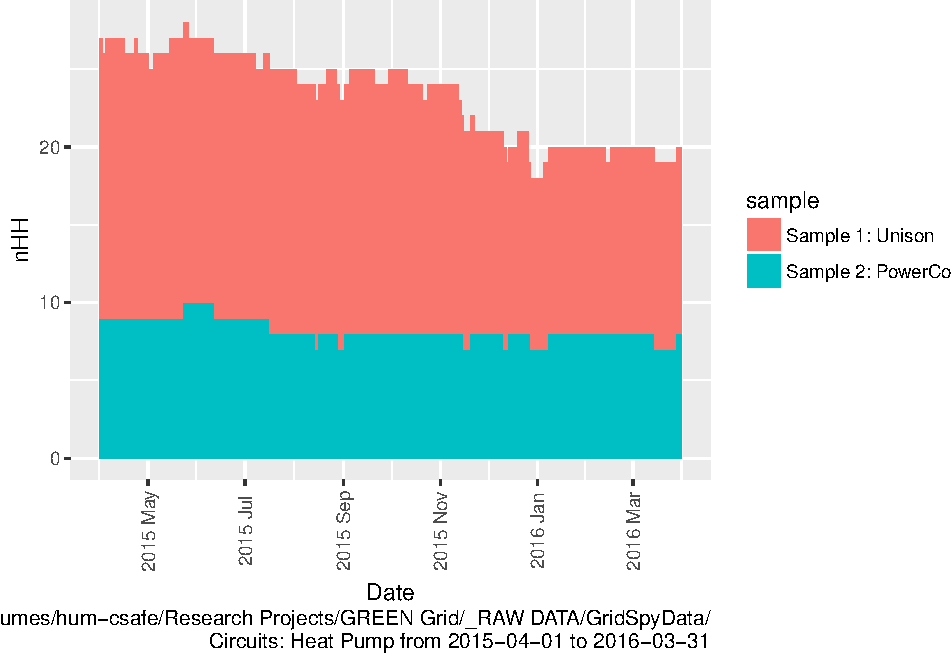
\includegraphics{ggProfile_Heat Pump_2015-04-01_2016-03-31_files/figure-latex/liveDataHouseholds-1.pdf}

The following table summarises the Heat Pump data. Any surprises?

\begin{Shaded}
\begin{Highlighting}[]
\NormalTok{t <-}\StringTok{ }\KeywordTok{summary}\NormalTok{(gs1MinDT)}
\KeywordTok{kable}\NormalTok{(}\DataTypeTok{caption =} \KeywordTok{paste0}\NormalTok{(}\StringTok{"Summary of "}\NormalTok{, circuitPattern, }\StringTok{" circuits"}\NormalTok{), t)}
\end{Highlighting}
\end{Shaded}

Summary of Heat Pump circuits

\begin{verbatim}
 hhID </th>
\end{verbatim}

r\_dateTime

circuit

\begin{verbatim}
 powerW </th>
\end{verbatim}

obsHourMin

Length:14252439

Length:14252439

Length:14252439

Min. : -655.00

Length:14252439

Class :character

Class :character

Class :character

1st Qu.: 0.00

Class :character

Mode :character

Mode :character

Mode :character

Median : 0.00

Mode :character

NA

NA

NA

Mean : 147.90

NA

NA

NA

NA

3rd Qu.: 61.23

NA

NA

NA

NA

Max. :27759.00

NA

We seem to have some negative powerW values and at least one very large
power value.

Nasty surprises often lurk in histograms\ldots{} The following histogram
shows all observations.

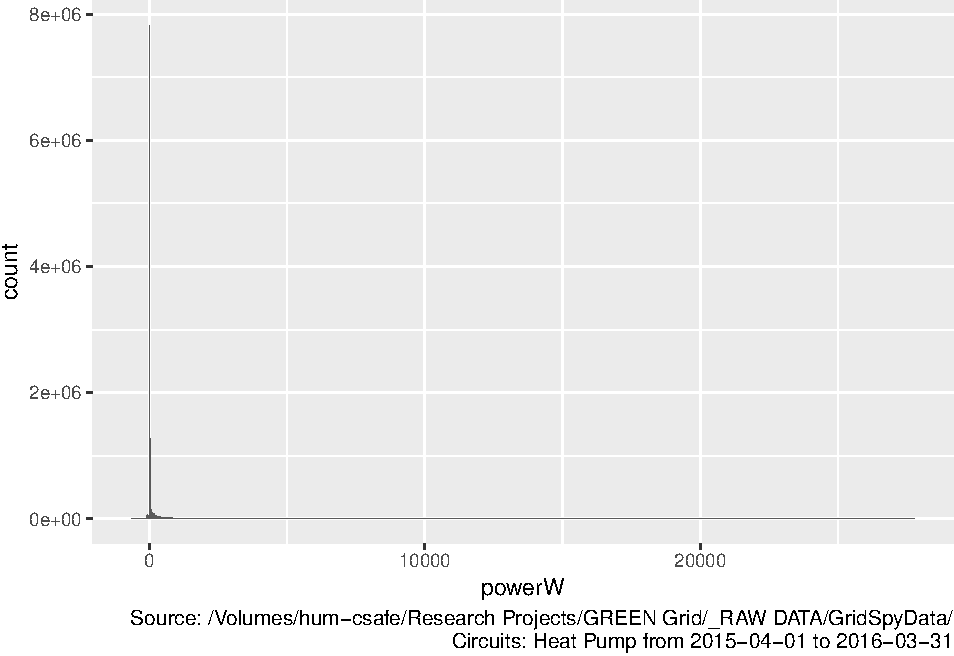
\includegraphics{ggProfile_Heat Pump_2015-04-01_2016-03-31_files/figure-latex/histo full-1.pdf}

The next shows the histogram for powerW \textless{} 1000W\ldots{}

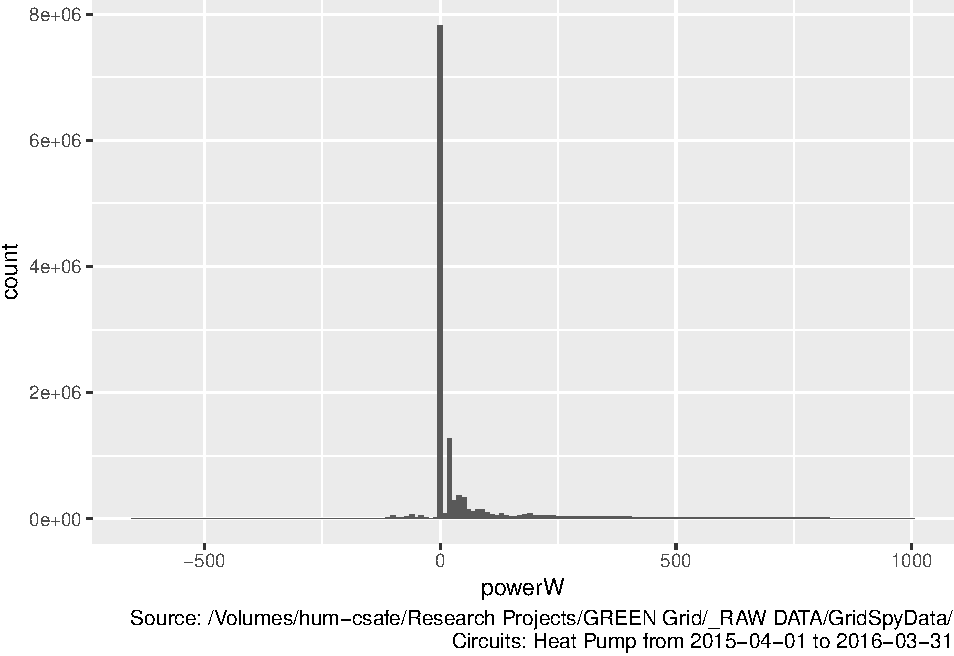
\includegraphics{ggProfile_Heat Pump_2015-04-01_2016-03-31_files/figure-latex/histo power under 1000-1.pdf}

\begin{quote}
There are a lot of zeros (as we'd expect) but why are there negative
values?
\end{quote}

\section{Heat Pump profiles}\label{heat-pump-profiles}

This section produces the profiles as one for each HH but averaged over
each season. Data is kept at 1 minute intervals. Note definition of
season below\ldots{}

\begin{Shaded}
\begin{Highlighting}[]
\CommentTok{# add season}
\NormalTok{gs1MinDT <-}\StringTok{ }\NormalTok{gs1MinDT[, month }\OperatorTok{:}\ErrorTok{=}\StringTok{ }\NormalTok{lubridate}\OperatorTok{::}\KeywordTok{month}\NormalTok{(r_dateTime, }\DataTypeTok{label =} \OtherTok{TRUE}\NormalTok{)]}
\NormalTok{gs1MinDT <-}\StringTok{ }\NormalTok{gs1MinDT[, season }\OperatorTok{:}\ErrorTok{=}\StringTok{ "Summer"}\NormalTok{]}
\NormalTok{gs1MinDT <-}\StringTok{ }\NormalTok{gs1MinDT[, season }\OperatorTok{:}\ErrorTok{=}\StringTok{ }\KeywordTok{ifelse}\NormalTok{(month }\OperatorTok{==}\StringTok{ "Mar"} \OperatorTok{|}
\StringTok{                                              }\NormalTok{month }\OperatorTok{==}\StringTok{ "Apr"} \OperatorTok{|}
\StringTok{                                              }\NormalTok{month }\OperatorTok{==}\StringTok{ "May"}\NormalTok{, }\StringTok{"Autumn"}\NormalTok{, season)]}
\NormalTok{gs1MinDT <-}\StringTok{ }\NormalTok{gs1MinDT[, season }\OperatorTok{:}\ErrorTok{=}\StringTok{ }\KeywordTok{ifelse}\NormalTok{(month }\OperatorTok{==}\StringTok{ "Jun"} \OperatorTok{|}
\StringTok{                                              }\NormalTok{month }\OperatorTok{==}\StringTok{ "Jul"} \OperatorTok{|}
\StringTok{                                              }\NormalTok{month }\OperatorTok{==}\StringTok{ "Aug"}\NormalTok{, }\StringTok{"Winter"}\NormalTok{, season)]}
\NormalTok{gs1MinDT <-}\StringTok{ }\NormalTok{gs1MinDT[, season }\OperatorTok{:}\ErrorTok{=}\StringTok{ }\KeywordTok{ifelse}\NormalTok{(month }\OperatorTok{==}\StringTok{ "Sep"} \OperatorTok{|}
\StringTok{                                              }\NormalTok{month }\OperatorTok{==}\StringTok{ "Oct"} \OperatorTok{|}
\StringTok{                                              }\NormalTok{month }\OperatorTok{==}\StringTok{ "Nov"}\NormalTok{, }\StringTok{"Spring"}\NormalTok{, season)]}
\end{Highlighting}
\end{Shaded}

\subsection{Profile plots: means per
household}\label{profile-plots-means-per-household}

This section shows a plot of mean profiles for each household by season.

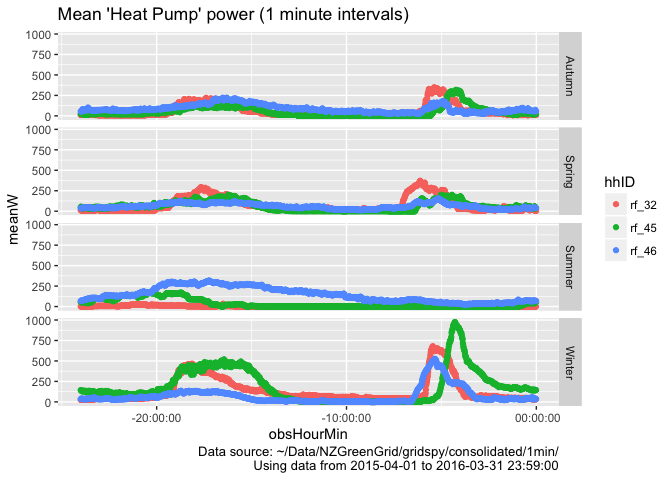
\includegraphics{ggProfile_Heat Pump_2015-04-01_2016-03-31_files/figure-latex/profiles per household by season-1.pdf}

\begin{verbatim}
## [1] "Saving plot to Heat Pump_2015-04-01_2016-03-31_byHouseholdSeasonalProfilePlot.png"
\end{verbatim}

\begin{verbatim}
## [1] "Saving profile data used to build this plot to: /Volumes/hum-csafe/Research Projects/GREEN Grid/Clean_data/safe/gridSpy/1min/profiles/Heat Pump_2015-04-01_2016-03-31_byHouseholdSeasonalProfiles.csv..."
\end{verbatim}

\begin{verbatim}
## [1] "Gzipped /Volumes/hum-csafe/Research Projects/GREEN Grid/Clean_data/safe/gridSpy/1min/profiles/Heat Pump_2015-04-01_2016-03-31_byHouseholdSeasonalProfiles.csv"
\end{verbatim}

Summary of household level mean profiles for Heat Pump

\begin{verbatim}
 hhID </th>
\end{verbatim}

obsHourMin

\begin{verbatim}
season </th>
\end{verbatim}

\begin{verbatim}
 meanW </th>
\end{verbatim}

Length:151200

Length:151200

Length:151200

Min. : -2.422

Class :character

Class :character

Class :character

1st Qu.: 12.347

Mode :character

Mode :character

Mode :character

Median : 58.538

NA

NA

NA

Mean : 149.354

NA

NA

NA

3rd Qu.: 195.366

NA

NA

NA

Max. :1778.669

As we can see there is considerable variation between households in both
the level and timing of heat pump demand.

Note that the code saves a high definition version of the plot and the
profiles for future re-use.

The .csv.gz file can be loaded using the following code:

\begin{itemize}
\tightlist
\item
  \texttt{df\ \textless{}-\ readr::read\_csv("/Volumes/hum-csafe/Research\ Projects/GREEN\ Grid/Clean\_data/safe/gridSpy/1min/profiles/Heat\ Pump\_2015-04-01\_2016-03-31\_byHouseholdSeasonalProfiles.csv.gz")}
  or
\item
  \texttt{dt\ \textless{}-\ data.table::as.data.table(readr::read\_csv("/Volumes/hum-csafe/Research\ Projects/GREEN\ Grid/Clean\_data/safe/gridSpy/1min/profiles/Heat\ Pump\_2015-04-01\_2016-03-31\_byHouseholdSeasonalProfiles.csv.gz"))}
  if you prefer \texttt{data.table}
\end{itemize}

\subsection{Profile plots: overall household
mean}\label{profile-plots-overall-household-mean}

This section shows a plot of mean and median profiles across all
household by season. The mean profile also shows the level of variance
by plotting error bars at +/- 1 s.d.

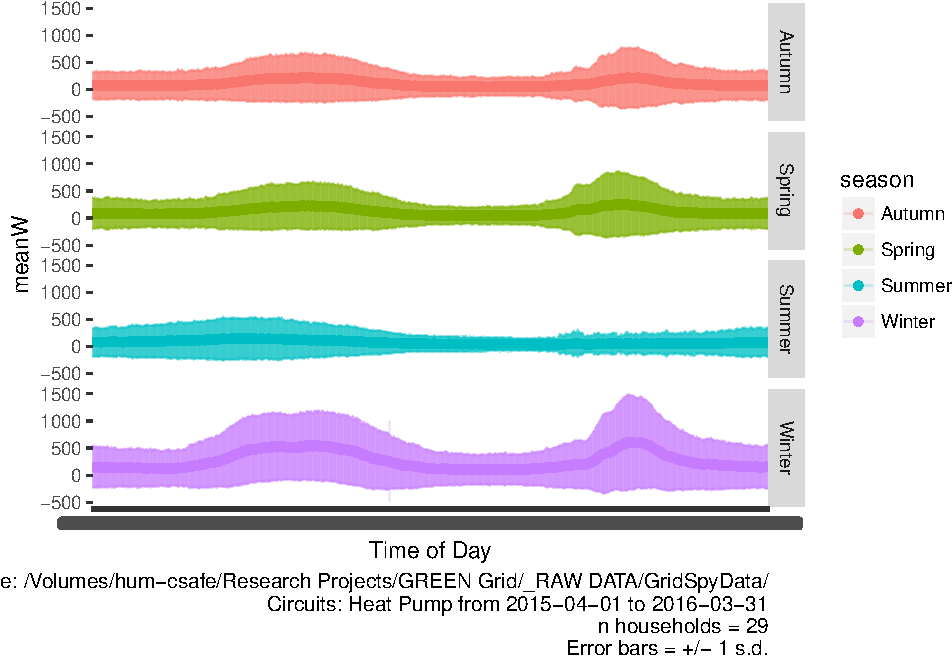
\includegraphics{ggProfile_Heat Pump_2015-04-01_2016-03-31_files/figure-latex/overall profiles by season-1.pdf}

\begin{verbatim}
## [1] "Saving plot to Heat Pump_2015-04-01_2016-03-31_overallMeanSeasonalProfilePlot.png"
\end{verbatim}

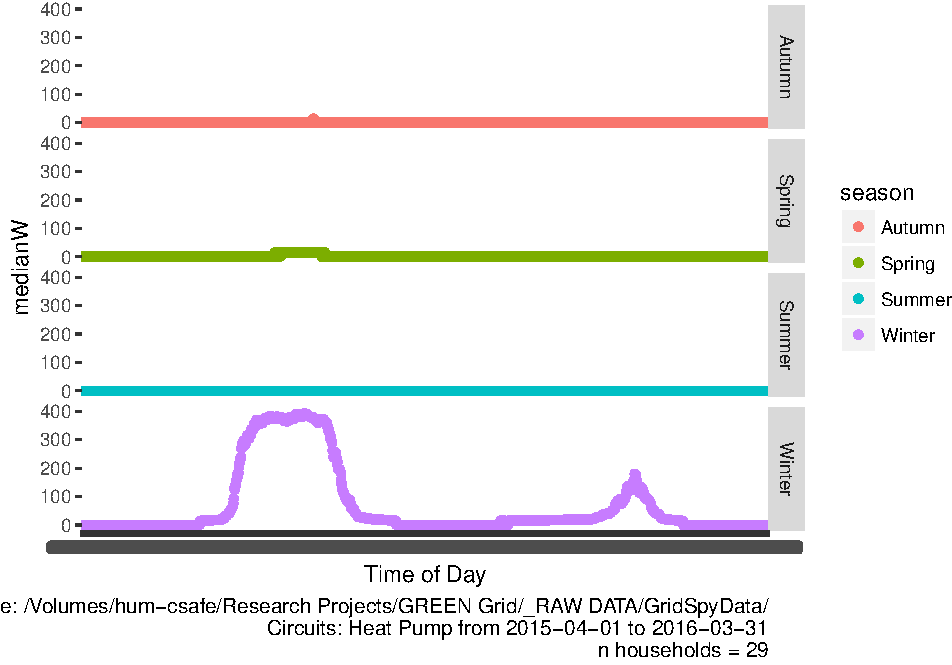
\includegraphics{ggProfile_Heat Pump_2015-04-01_2016-03-31_files/figure-latex/overall profiles by season-2.pdf}

\begin{verbatim}
## [1] "Saving plot to Heat Pump_2015-04-01_2016-03-31_overallMedianSeasonalProfilePlot.png"
\end{verbatim}

\begin{verbatim}
## [1] "Saving profile data used to build this plot to: /Volumes/hum-csafe/Research Projects/GREEN Grid/Clean_data/safe/gridSpy/1min/profiles/Heat Pump_2015-04-01_2016-03-31_overallSeasonalProfiles.csv..."
\end{verbatim}

\begin{verbatim}
## [1] "Gzipped /Volumes/hum-csafe/Research Projects/GREEN Grid/Clean_data/safe/gridSpy/1min/profiles/Heat Pump_2015-04-01_2016-03-31_overallSeasonalProfiles.csv"
\end{verbatim}

Summary of overall profiles for Heat Pump

obsHourMin

\begin{verbatim}
season </th>
\end{verbatim}

\begin{verbatim}
 meanW </th>
\end{verbatim}

\begin{verbatim}
medianW </th>
\end{verbatim}

\begin{verbatim}
  nObs </th>
\end{verbatim}

\begin{verbatim}
  sdW </th>
\end{verbatim}

Length:5760

Length:5760

Min. : 34.99

Min. : 0.00

Min. :2150

Min. :101.0

Class :character

Class :character

1st Qu.: 71.88

1st Qu.: 0.00

1st Qu.:2402

1st Qu.:234.3

Mode :character

Mode :character

Median :104.76

Median : 0.00

Median :2518

Median :298.6

NA

NA

Mean :143.52

Mean : 17.09

Mean :2474

Mean :329.8

NA

NA

3rd Qu.:174.71

3rd Qu.: 0.00

3rd Qu.:2599

3rd Qu.:407.1

NA

NA

Max. :613.89

Max. :392.55

Max. :2688

Max. :879.1

The difference between the mean and median plots is instructive - it
suggests that the mean plots for summer are skewed by a few higher heat
pump-using households.

The plots could be repeated or re-facted e.g.~by household size.

As before, the code saves a high definition version of the plot and the
profiles for future re-use.

\section{Runtime}\label{runtime}

Analysis completed in 621.26 seconds ( 10.35 minutes) using
\href{https://cran.r-project.org/package=knitr}{knitr} in
\href{http://www.rstudio.com}{RStudio} with R version 3.5.0 (2018-04-23)
running on x86\_64-apple-darwin15.6.0.

\section{R environment}\label{r-environment}

R packages used:

\begin{itemize}
\tightlist
\item
  base R - for the basics (R Core Team 2016)
\item
  data.table - for fast (big) data handling (Dowle et al. 2015)
\item
  lubridate - date manipulation (Grolemund and Wickham 2011)
\item
  ggplot2 - for slick graphics (Wickham 2009)
\item
  readr - for csv reading/writing (Wickham, Hester, and Francois 2016)
\item
  dplyr - for select and contains (Wickham and Francois 2016)
\item
  progress - for progress bars (Csárdi and FitzJohn 2016)
\item
  knitr - to create this document \& neat tables (Xie 2016)
\item
  kableExtra - for extra neat tables (Zhu 2018)
\item
  nzGREENGrid - for local NZ GREEN Grid project utilities
\end{itemize}

Session info:

\begin{verbatim}
## R version 3.5.0 (2018-04-23)
## Platform: x86_64-apple-darwin15.6.0 (64-bit)
## Running under: macOS High Sierra 10.13.5
## 
## Matrix products: default
## BLAS: /System/Library/Frameworks/Accelerate.framework/Versions/A/Frameworks/vecLib.framework/Versions/A/libBLAS.dylib
## LAPACK: /Library/Frameworks/R.framework/Versions/3.5/Resources/lib/libRlapack.dylib
## 
## locale:
## [1] en_GB.UTF-8/en_GB.UTF-8/en_GB.UTF-8/C/en_GB.UTF-8/en_GB.UTF-8
## 
## attached base packages:
## [1] stats     graphics  grDevices utils     datasets  methods   base     
## 
## other attached packages:
## [1] rmarkdown_1.9     kableExtra_0.9.0  knitr_1.20        readr_1.1.1      
## [5] ggplot2_2.2.1     dplyr_0.7.5       data.table_1.11.2 nzGREENGrid_0.1.0
## 
## loaded via a namespace (and not attached):
##  [1] progress_1.1.2      tinytex_0.5         tidyselect_0.2.4   
##  [4] reshape2_1.4.3      purrr_0.2.4         splines_3.5.0      
##  [7] lattice_0.20-35     colorspace_1.3-2    htmltools_0.3.6    
## [10] viridisLite_0.3.0   yaml_2.1.19         base64enc_0.1-3    
## [13] survival_2.42-3     rlang_0.2.0         pillar_1.2.2       
## [16] foreign_0.8-70      glue_1.2.0          RColorBrewer_1.1-2 
## [19] readxl_1.1.0        bindrcpp_0.2.2      bindr_0.1.1        
## [22] plyr_1.8.4          stringr_1.3.1       munsell_0.4.3      
## [25] gtable_0.2.0        cellranger_1.1.0    rvest_0.3.2        
## [28] htmlwidgets_1.2     evaluate_0.10.1     labeling_0.3       
## [31] latticeExtra_0.6-28 htmlTable_1.11.2    highr_0.6          
## [34] Rcpp_0.12.17        acepack_1.4.1       checkmate_1.8.5    
## [37] backports_1.1.2     scales_0.5.0        Hmisc_4.1-1        
## [40] gridExtra_2.3       hms_0.4.2           digest_0.6.15      
## [43] stringi_1.2.2       grid_3.5.0          rprojroot_1.3-2    
## [46] tools_3.5.0         magrittr_1.5        lazyeval_0.2.1     
## [49] tibble_1.4.2        cluster_2.0.7-1     Formula_1.2-3      
## [52] pkgconfig_2.0.1     Matrix_1.2-14       xml2_1.2.0         
## [55] prettyunits_1.0.2   lubridate_1.7.4     assertthat_0.2.0   
## [58] httr_1.3.1          rstudioapi_0.7      rpart_4.1-13       
## [61] R6_2.2.2            nnet_7.3-12         compiler_3.5.0
\end{verbatim}

\section*{References}\label{references}
\addcontentsline{toc}{section}{References}

\hypertarget{refs}{}
\hypertarget{ref-progress}{}
Csárdi, Gábor, and Rich FitzJohn. 2016. \emph{Progress: Terminal
Progress Bars}. \url{https://CRAN.R-project.org/package=progress}.

\hypertarget{ref-data.table}{}
Dowle, M, A Srinivasan, T Short, S Lianoglou with contributions from R
Saporta, and E Antonyan. 2015. \emph{Data.table: Extension of
Data.frame}. \url{https://CRAN.R-project.org/package=data.table}.

\hypertarget{ref-lubridate}{}
Grolemund, Garrett, and Hadley Wickham. 2011. ``Dates and Times Made
Easy with lubridate.'' \emph{Journal of Statistical Software} 40 (3):
1--25. \url{http://www.jstatsoft.org/v40/i03/}.

\hypertarget{ref-baseR}{}
R Core Team. 2016. \emph{R: A Language and Environment for Statistical
Computing}. Vienna, Austria: R Foundation for Statistical Computing.
\url{https://www.R-project.org/}.

\hypertarget{ref-ggplot2}{}
Wickham, Hadley. 2009. \emph{Ggplot2: Elegant Graphics for Data
Analysis}. Springer-Verlag New York. \url{http://ggplot2.org}.

\hypertarget{ref-dplyr}{}
Wickham, Hadley, and Romain Francois. 2016. \emph{Dplyr: A Grammar of
Data Manipulation}. \url{https://CRAN.R-project.org/package=dplyr}.

\hypertarget{ref-readr}{}
Wickham, Hadley, Jim Hester, and Romain Francois. 2016. \emph{Readr:
Read Tabular Data}. \url{https://CRAN.R-project.org/package=readr}.

\hypertarget{ref-knitr}{}
Xie, Yihui. 2016. \emph{Knitr: A General-Purpose Package for Dynamic
Report Generation in R}. \url{https://CRAN.R-project.org/package=knitr}.

\hypertarget{ref-kableExtra}{}
Zhu, Hao. 2018. \emph{KableExtra: Construct Complex Table with 'Kable'
and Pipe Syntax}. \url{https://CRAN.R-project.org/package=kableExtra}.


\end{document}
